% 
%  ArchitectureChapter.tex
%  ThesisISEL
%  
%  Created by Sana on 2023/02/05.
%

\chapter{Architecture}
\label{cha:architecture_chapter}

In this section, we will discuss the proposed architecture for the approach taken in this work. This includes the scope, data sources, data representation choices, weaknesses, and the chosen target programming language selected for our case study.

% ================
% = Target programming language =
% ================
\section{Selecting Java as target programming language} % (fold)
\label{sec: target_programming_language}


Despite Java is considered a relatively safe language, there are still several ways to attack and access private information if we misuse it, leading to vulnerabilities such as Command injection and cross-site scripting attacks. Fred Long \cite{10.5555/2536828} asserts that Java is secure if is used properly, but engineers can misuse it or improperly implement it. A simple programming mistake can leave a java application vulnerable to unauthorized data access, unauthorized updates or even loss of data, and application crashes leading to denial-of-service attacks.

Among all the vulnerabilities detected in Java applications, those arising from \textbf{unchecked input} are widely acknowledged as the most prevalent \cite{OWASP_TOP_TEN_2004}.

To exploit unchecked input, an attacker needs to achieve two goals: 

\begin{itemize}
\item  Inject malicious data into application;
\item  Manipulate applications using malicious codes such as Command injection or Cross-site scripting.
\end{itemize}

All those types of attacks listed above are made possible by user input that has not been
(properly) validated.\\

This work focuses in source code written in Java. The next subsections will delineate some typical vulnerabilities that are considered in our study case.  It's important to note that all the provided examples are deliberately kept simple, solely intended to illustrate the overarching concept, and the actual exploitation of these vulnerabilities is considerably more intricate in practical scenarios.


\section{NULL Pointer Deference vulnerability} % (fold)
\label{sub: NULL_Pointer_Dereference}

A pointer deference \cite{ImmuniWeb2012, CVE476} is a programming language data variable that references a location in memory. After the value of the location is obtained by the pointer, this pointer is considered dereferenced. It is a widespread vulnerability that occurs whenever an executing program attempts to deference a null pointer \cite{WENHUI_JIN12021}, i.e., a pointer which references a null location. 

\begin{figure}[ht]
	\centering
	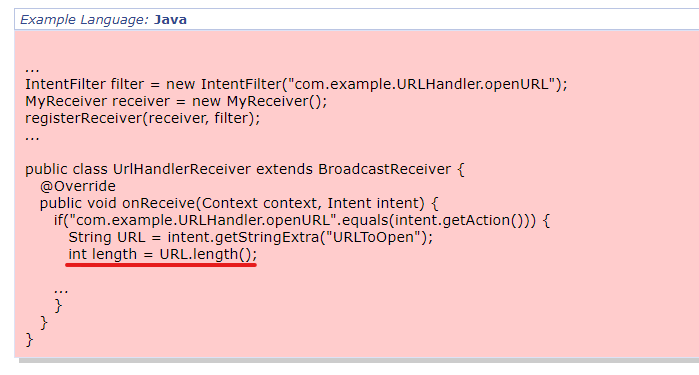
\includegraphics[width=0.90\textwidth]{NPD_JAVA2}
	  \caption{Null pointer deference java example}
  \label{fig:java_npd}
\end{figure}

Figure \ref{fig:java_npd} depicts a Null pointer dereference example. The code snippet is from an Android application that has registered to handle a URL when sent an intent. The application code exemplified assumes the URL (Uniform Resource Locator) will always be included in the intent. When the URL is not present, the call to \(getStringExtra()\) will return null, thus causing a null pointer exception when length() is called.

NULL Pointer Dereference vulnerability can be exploited by hackers to maliciously crash a process to cause a denial of service or execute an arbitrary code under specific conditions. This typical taint-style vulnerability requires an accurate data dependency analysis to trace whether a source is propagated to a sensitive sink without proper sanitization \cite{WENHUI_JIN12021}. This vulnerability is mostly used to crash a kernel or process to cause a denial-of-service attack.

NULL Pointer Dereference has been included in "CWE Top 25 Most Dangerous Software Weaknesses" published by the CWE website \cite{CVE_TOP25} every year. The ranking scores are calculated by considering both the number of reported vulnerabilities and the potential severity of a vulnerability. An attacker can exploit it indirectly to trigger an arbitrary code execution or bypass authentication \cite{Pietro_Oliva2023}, in specific situations. For example, CVE-2021-42264 \cite{CVE_2021_42264} reported that \textit{Adobe Premiere Pro 15.4.1} (and earlier) is affected by a Null pointer dereference vulnerability when parsing a specially crafted file. An unauthenticated attacker could leverage this vulnerability to achieve an application denial-of-service in the context of the current user. Exploitation of this issue requires user interaction in that a victim must open a malicious file.

The following  points may be considered as potential mitigations:
\begin{itemize}
\item By performing sanity checks on all pointers that could have been modified, nearly all NULL pointer references can be prevented;
\item  Check the results of the returned value of functions to verify that this value is not NULL before using it;
\item  Perform input validation on variables and data stores that may receive input from an external source and apply input validation to make sure that they are only initialized to expected values;
\item  Explicitly initialize all variables and other data stores during declaration or before the first usage.
\end{itemize}

% ection NULL_Pointer_Dereference(end)

\section{Command Injection vulnerabilities} % (fold)
\label{sub: Command_Injection_vulnerabilities}

Command Injection is a general term for attack types which consist of injecting commands that are consequently executed by the vulnerable application. This type of attacks is considered as a major security threat which in fact,  is  classified  as  No. 3  on  the  2021  \gls{owasp} Top  Ten  web  security  risks \cite{OWASP_TOP_TEN2021}.

Command injection vulnerabilities typically occur when data enters the application from an untrusted source. The data is part of a string that is executed as a command by the application. By executing the command, the application gives an attacker a privilege or capability that the attacker would not otherwise have.

According to the \gls{owasp} \cite{Weilin_Zhong2023}, Command injection is an attack in which the goal is execution of arbitrary commands on the host operating system via a vulnerable application. Command injection attacks are possible when an application passes unsafe user supplied data (forms, cookies, HTTP headers, etc.) to a system shell. In this attack, the attacker-supplied operating system commands are usually executed with the privileges of the vulnerable application. Command injection attacks are possible largely due to insufficient input validation.

The impact of command injection attacks may vary from loss of data confidentiality and integrity to unauthorized remote access to the system that hosts the vulnerable application. In particular, an attacker can gain access to resources that he/she does not have privileges to directly accessing them, such as system files that include sensitive data (e.g., passwords). An attacker can perform various malicious actions to the vulnerable system, such as delete files or add new system users for remote access and persistence. An example of a real, infamous command injection vulnerability that clearly describe the threats of this type of code injection was the recently discovered (i.e., disclosed in 2014) Shellshock bug \cite{Shellshock}.

Command injections vulnerabilities may be present in applications which accept and process system commands from the user input. The purpose of a command injection attack is the injection of an operating system command through the data input to the vulnerable application which in turn executes the injected command (see Figure ~\ref{fig:CIJAVA}). 

\begin{figure}[ht]
	\centering
	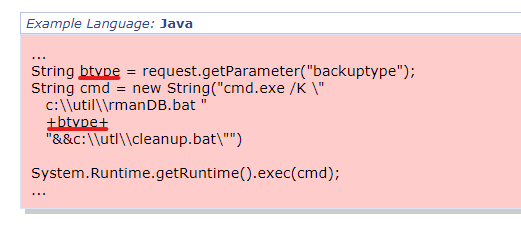
\includegraphics[width=0.90\textwidth]{CI_JAVA2}
	  \caption{Command injection vulnerability - Java example}
  \label{fig:CIJAVA}
\end{figure}
%https://cwe.mitre.org/data/definitions/77.html

Figure ~\ref{fig:CIJAVA} portrays a Command Injection Vulnerability situation in Java code excerpt. The following code is taken from an administrative web application designed to enable users to initiate a backup of an Oracle database using a batch-file wrapper around the \textit{rman} utility and subsequently execute a \textit{cleanup.bat} script to remove certain temporary files. The script \textit{rmanDB.bat} accepts a single command-line parameter that specifies the type of backup to be performed. Since access to the database is restricted, the application executes the backup as a privileged user.

The issue here is that the program lacks validation for the \texttt{backuptype} parameter provided by the user. Typically, the \texttt{Runtime.exec()} function does not execute multiple commands. However, in this case, the program first invokes the \texttt{cmd.exe} shell to run multiple commands with a single call to \texttt{Runtime.exec()}. Once the shell is invoked, it will execute multiple commands separated by double ampersands \texttt{\&\&}. If an attacker submits a string in the form of \texttt{\& del c:\textbackslash dbms\textbackslash .}, the application will execute this injected command in addition to the commands specified by the program. Due to the application's nature, it runs with the privileges required for interacting with the database. As a result, any injected command by the attacker will also run with these elevated privileges.

There are many types of code injections attacks including Command injections, SQL Injections, Cross Site Scripting, XPath Injections and LDAP (Lightweight Directory Access Protocol) Injection \cite{Anastasios_Stasinopoulos2015}. In this work, we will exclusively deal with command injection attacks. Command injections \cite{Anastasios_Stasinopoulos2015} are prevalent in any application, regardless of the operating system hosting the application or the programming language in which the application is developed. Consequently, they have also been discovered in web applications hosted on web servers, whether they are Windows-based or Unix-based.

The following  points may be considered as potential mitigation:
\begin{itemize}
\item  Use library calls, if possible, rather than external processes to recreate the desired functionality. Ensure that all external commands called from the program are statically created;
\item  Assign permissions to the software system that prevents the user from accessing/opening privileged files;
\item  Consider all potentially relevant properties, including length, type of input, when performing input validation.
\end{itemize}

% subsection Command_Injection_vulnerabilities(end)

% section Selected_vulnerabilities (end)

\section{Proposed Architecture} % (fold)
\label{sec: Proposed_Architecture}

Up to this point, we have been describing the chosen target programming language selected for our case study. The next section will outline the proposed architecture for the approach we have taken.

We proposed an approach inspired by a research that used data-flow analysis and machine learning to detect SQLi and XSS vulnerabilities in PHP software code \cite{Kronjee2018}. In the proposed architecture, presented in the Figure \ref{fig:archquitecture}, we diverged from the utilization of XSS and SQLi vulnerabilities. Instead, we opted for Java as the target programming language and chose to focus on detecting weaknesses such as NULL Pointer Deference and Command Injection. This work proposes a tool based on a static analysis and machine learning for finding vulnerabilities caused by unchecked input.

The primary contribution of this research comprises the development of a prototype capable of identifying vulnerable Java source code through the application of a probabilistic classifier and features derived from static code analysis. To achieve this, we will compile a dataset for training and testing our classifiers. This dataset will be sourced from the National Vulnerability Database (NVD) \cite{NVD2023} and the Software Assurance Metrics And Tool Evaluation (SAMATE) project \cite{SAMATE2023}.

\begin{figure}[ht]
	\centering
	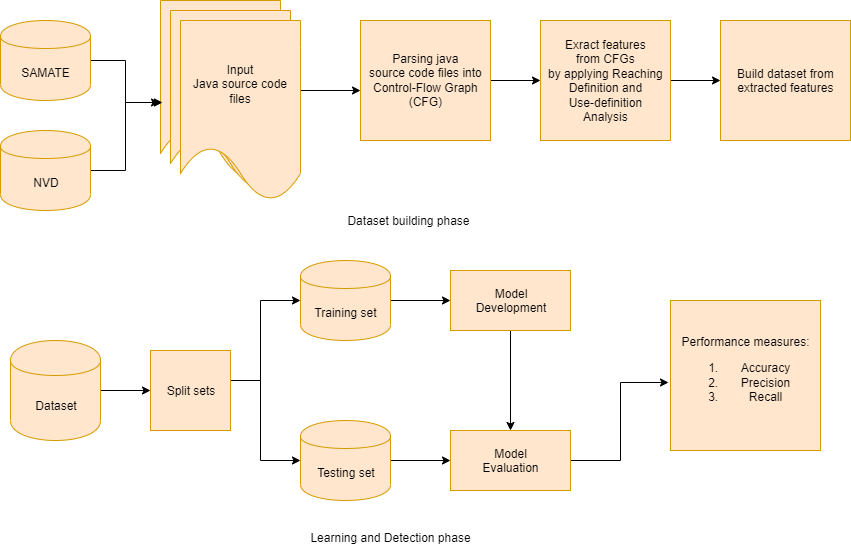
\includegraphics[width=0.90\textwidth]{Architecture3}
	  \caption{A high-level flow of proposed architecture}
  \label{fig:archquitecture}
\end{figure}

As depicted in Figure \ref{fig:archquitecture}, the project will be organized into two primary phases. The initial phase comprises dataset building, wherein we will generate Control Flow Graphs (CFGs) from Java source files and extract corresponding features. Subsequently, the following phase involves learning and detection. During this phase, we will divide the dataset into two subsets: the training set, designated for model training, and the testing set, utilized for model assessment.

Similarly to the approach undertaken by Kronjee et al \cite{Kronjee2018}, we intend to employ the Abstract Syntax Tree (\gls{ast}) and control-flow graph as the foundational sources for extracting features. We are of the opinion that the \gls{ast} could provide substantial information about the code, which could be highly valuable, including discerning whether a token represents a function or a variable, as well as identifying the functions applied to specific variables.

Reaching definition and taint analysis will be used to identify potential vulnerabilities. Utilizing the \gls{ast}, we can determine that a variable is being used as a parameter for a call to function. This means that we can provide these functions and their respective argument values (variables) as features to our probabilistic classifier. By applying this method, our machine learning algorithm will learn which function is likely to be a potentially vulnerable function given enough samples. To determine if a function is applied to a variable, we can construct a \gls{cfg}, from the \gls{ast}. By considering the entire preceding execution path, we can use the invocation of functions in that path as a feature.

When applying taint analysis, the \gls{ast} can provide us information if a variable has been assigned using a literal value, like a number or a string. In that case, the data is from a trusted source and the variable is untainted. However, if the variable's value is derived from a source like another variable or a function—especially if this source isn't a literal—the variable must be treated as tainted. Subsequently, anything that is set using this variable must be also considered tainted as well. By using this approach we can determine whether a variable contains data from a specific source and whether  it's tainted or untainted. 

To facilitate feature extraction, we require a parser capable of translating code into an \gls{ast}, subsequently enabling the construction of a \gls{cfg}. To accomplish this, we will utilize the "spoon-control-flow" component \cite{OW2_SPOON}. This module offers the capability to generate both control-flow and data-flow graphs for a Java program, relying on its \gls{ast} that is also created using the Spoon library. Subsequently, we will implement reaching definitions analysis and use-definition techniques to extract features from the \gls{ast}.

To programmatically determine the reaching definitions from our \gls{ast}, we used the algorithm described in Section \ref{sec:Reaching_definitions_analysis}, based on the description from \cite{Alfred_V2007}. The referenced book, primarily deals with code blocks. However, in our specific scenario, we have modified the implementation. This adjustment was necessary due to complexities in implementation, leading us to focus on control-flow nodes rather than traditional code blocks.

After building the Reaching Definitions sets,  our next step involves establishing the Use-Definition (\gls{ud}) chains for each definition. \gls{ud} chains comprise a utilization of a variable U, and all the definitions D of that variable that can reach that use without any other intervening definitions in between.

For each node within the \gls{cfg} of the program, our objective is to determine which functions may have been used in the paths to that nodes. We consider the invocation of functions as features, hence, in our feature set, we use \gls{ud} chains to create new features. We consider each node to be a sample that can potentially be categorized as either vulnerable or not vulnerable. 

As explained in Section \ref{sec:Use_definition_Analysis}, in order to detect vulnerabilities, there needs to be a potentially vulnerable function and a lack of sanitization, which usually comes in the form of a function as well.By utilizing the presence of functions as features, we can derive a feature set wherein all functions invoked using values from potentially untainted variables serve as our features.

